\documentclass[
  bibliography=totoc,     % Literatur im Inhaltsverzeichnis
  captions=tableheading,  % Tabellenüberschriften
  titlepage=firstiscover, % Titelseite ist Deckblatt
  parskip=half,
]{scrartcl}

% Paket float verbessern
\usepackage{scrhack}

% Warnung, falls nochmal kompiliert werden muss
\usepackage[aux]{rerunfilecheck}

% unverzichtbare Mathe-Befehle
\usepackage{amsmath}
% viele Mathe-Symbole
\usepackage{amssymb}
% Erweiterungen für amsmath
\usepackage{mathtools}

% Fonteinstellungen
\usepackage{fontspec}
\usepackage{dsfont}
% Latin Modern Fonts werden automatisch geladen
% Alternativ zum Beispiel:
%\setromanfont{Libertinus Serif}
%\setsansfont{Libertinus Sans}
%\setmonofont{Libertinus Mono}

% Wenn man andere Schriftarten gesetzt hat,
% sollte man das Seiten-Layout neu berechnen lassen
\recalctypearea{}

% deutsche Spracheinstellungen
\usepackage[main=ngerman]{babel}


\usepackage[
  math-style=ISO,    % ┐
  bold-style=ISO,    % │
  sans-style=italic, % │ ISO-Standard folgen
  nabla=upright,     % │
  partial=upright,   % ┘
  warnings-off={           % ┐
    mathtools-colon,       % │ unnötige Warnungen ausschalten
    mathtools-overbracket, % │
  },                       % ┘
]{unicode-math}

% traditionelle Fonts für Mathematik
\setmathfont{Latin Modern Math}
% Alternativ zum Beispiel:
%\setmathfont{Libertinus Math}

\setmathfont{XITS Math}[range={scr, bfscr}]
\setmathfont{XITS Math}[range={cal, bfcal}, StylisticSet=1]

% Zahlen und Einheiten
\usepackage[
  locale=DE,                   % deutsche Einstellungen
  separate-uncertainty=true,   % immer Fehler mit \pm
  per-mode=symbol-or-fraction, % / in inline math, fraction in display math
]{siunitx}

% chemische Formeln
\usepackage[
  version=4,
  math-greek=default, % ┐ mit unicode-math zusammenarbeiten
  text-greek=default, % ┘
]{mhchem}

% richtige Anführungszeichen
\usepackage[autostyle]{csquotes}

% schöne Brüche im Text
\usepackage{xfrac}

% Standardplatzierung für Floats einstellen
\usepackage{float}
\floatplacement{figure}{htbp}
\floatplacement{table}{htbp}

% Floats innerhalb einer Section halten
\usepackage[
  section, % Floats innerhalb der Section halten
  below,   % unterhalb der Section aber auf der selben Seite ist ok
]{placeins}

% Seite drehen für breite Tabellen: landscape Umgebung
\usepackage{pdflscape}

% Captions schöner machen.
\usepackage[
  labelfont=bf,        % Tabelle x: Abbildung y: ist jetzt fett
  font=small,          % Schrift etwas kleiner als Dokument
  width=0.9\textwidth, % maximale Breite einer Caption schmaler
]{caption}
% subfigure, subtable, subref
\usepackage{subcaption}

% Grafiken können eingebunden werden
\usepackage{graphicx}
% größere Variation von Dateinamen möglich
\usepackage{grffile}

% schöne Tabellen
\usepackage{booktabs}

% Verbesserungen am Schriftbild
\usepackage{microtype}

% Literaturverzeichnis
\usepackage[
  backend=biber,
]{biblatex}
% Quellendatenbank
\addbibresource{../bib/lit.bib}
\addbibresource{../bib/programme.bib}
\addbibresource{../bib/versuche.bib}

% Hyperlinks im Dokument
\usepackage[
  german,
  unicode,        % Unicode in PDF-Attributen erlauben
  pdfusetitle,    % Titel, Autoren und Datum als PDF-Attribute
  pdfcreator={},  % ┐ PDF-Attribute säubern
  pdfproducer={}, % ┘
]{hyperref}
% erweiterte Bookmarks im PDF
\usepackage{bookmark}

% Trennung von Wörtern mit Strichen
\usepackage[shortcuts]{extdash}

% Anpassbare Enumerates/Itemizes
\usepackage{enumitem}

\author{%
  Johannes Lamers\\%
  \href{mailto:johannes.lamers@edu.edu}{johannes.lamers@udo.edu}%
  \and%
  Sebastian Fischer\\%
  \href{mailto:sebastian5.fischer@udo.edu}{sebastian5.fischer@udo.edu}%
}
\publishers{TU Dortmund – Fakultät Physik}


\subject{V 61}
\title{Helium-Neon Laser}
\date{%
  Durchführung: 26.05.2021
  \hspace{3em}
  Abgabe: 22.09.2021
}
\usepackage{nicefrac}
\begin{document}

\maketitle
\thispagestyle{empty}
\tableofcontents
\newpage

%habs nur auskommentiert, damit das nicht jedes mal compiliert
\section{Zielsetzung}
\label{sec:Zielsetzung}

In diesem Versuch werden einige Eigenschaften und Bauteile der Mikrowellentechnik näher betrachtet. Dabei wird das Hohleiterfeld näher beleuchtet und auf seine Moden untersucht. Darüberhinaus werden Frequenz, Wellenlänge und Dämpung eines Dämpfungsgliedes bestimmt.
%Was ist das Ziel?
\section{Theorie}
\label{sec:Theorie}

\subsection{Grundprinzip}
Ein Laser (\textit{light amplification by stimulated emisson of radiation}) besteht hauptsächlich aus drei Komponenten.
Das \textit{aktive Medium}, welches von einer \textit{Energiepumpe} mit Energie gespeißt wird, sorgt für eine Besetzungsinversion zwischen mindestens zwei Energienivieaus im Medium. Der \textit{Resonator} sorgt schließlich über Hin- und Herreflektion dafür, dass das Licht möglichst häufig durch das aktive Medium hindurchgeht. Über einen Spiegel mit geringer Durchlässigkeit kann das Licht den Aufbau \ref{fig:auf} verlassen.

\begin{figure}
    \centering
    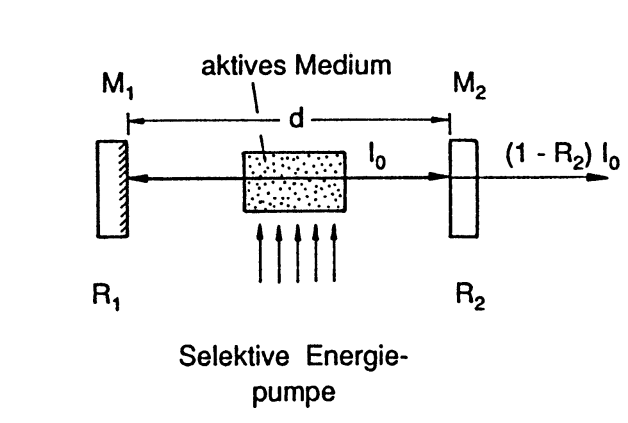
\includegraphics[width=8cm]{Bilder/Aufbau.PNG}
    \caption{Schematischer Aufbau des Lasers.\cite{Laserspektroskopie_1}}
    \label{fig:auf}
\end{figure}

\subsection{Das Aktive Medium}
Für die Funktionsweise eines Lasers sind drei Prozesse der Wechselwirkung zwischen Licht und Materie besonders wichtig:
\begin{itemize}
    \item Absorbtion:

    Trifft Licht auf ein Atom im Grundzustand, dessen Energie der Energiedifferenz zwischen Grundzustand und nächstem Energienivieau entspricht, wird dieses Licht aborbiert und das jeweilge Elektron wird auf das jeweilige Energienivieau gehoben. Dadurch geht das Atom in einen angeregten Zustand über.

    \item spontane Emission:

    Angeregte Atome fallen ohne äußeren Einfluss in ihren Grundzustande zurück und emittieren dabei ein Photon, dessen Energie wieder der Energiedifferenz zwischen den beiden Niveaus entspricht. Die spontane Emission geschieht zufällig und ist nur mit einer Emissionswahrscheinlichkeit geknüpft. 

    \item induzierte Emission:

    Trifft ein Photon auf ein angeregtes Atom, dessen Energie der Energiedifferenz zwischen zwei Zuständen entspricht, so geht das Atom in den jeweils geringeren Zustand über und emittiert dabei ein Photon gleicher Richtung, Polarisation und Wellenlänge.(Abbildung \ref{fig:ver})
\end{itemize}

\begin{figure}
    \centering
    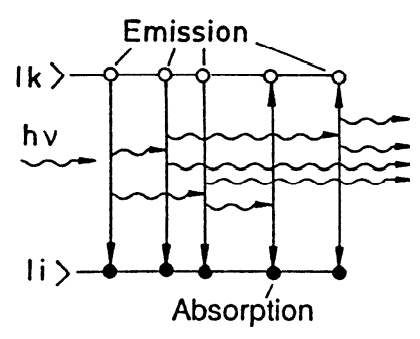
\includegraphics[width=6cm]{Bilder/verstaerkung.PNG}
    \caption{Prinzip der Verstärkung durch induzierte Emission.\cite{Laserspektroskopie_1}}
    \label{fig:ver}
\end{figure}

Damit es zu einer Verstärkung kommen kann, muss eine Besetzungsinversion im aktiven Medium erzeugt werden . Ohne äußeren Einfluss sind die Zustände der Atome im Medium gemäß der Boltzmann-Verteilung verteilt. Atome in Zuständen geringerer Energie kommen also häufiger vor, als welche in Zuständen höherer Energie. In dem Fall wäre die Erzeugung von induzierten Emission unwahrscheinlich und es käme zu keiner Verstärkung.
Die Energiepumpe sorgt dafür, dass ein Niveau höherer Energie häufiger Besetzt vorkommt, als ein Niveau niedrigerer Energie (Abbildung \ref{fig:inv}). Dadurch steigt die Wahrscheinlichkeit für jedes Photon im Medium, auf ein angeregtes Atom zu treffen und dadurch eine Emission zu induzieren. Je nach Wahl des aktiven Mediums ist auch die Energiedifferenz zwischen diesen beiden Niveaus eine andere. Dadurch ist das Medium entscheident für die Wellenlänge des vom Laser ausgestrahlten Lichtes.

\begin{figure}
    \centering
    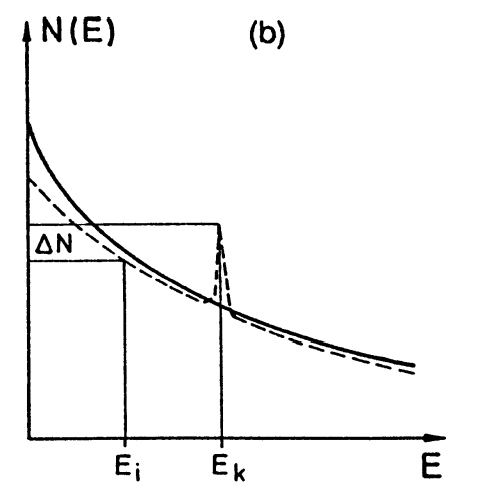
\includegraphics[width=6cm]{Bilder/Inversion.PNG}
    \caption{Verteilung der Zustände gemäß Boltzmann-Verteilung und gemäß Besetzungsinversion.\cite{Laserspektroskopie_1}}
    \label{fig:inv}
\end{figure}

\subsection{Stabilität des Resonators}
Der Resonator besteht aus zwei Spiegel, welche unterschiedliche Krümmungen besitzen können. Damit das Licht stabil im Resonator oszillieren kann, dürfen die Spiegel nur innerhalb gewisser Abstände zueinander sein. Sonst würde der zu große Verlust zu einem erliegen der Laser-Tätigkeit führen. In dem Fall (kleine Spiegel gegenüber dem Abstand) wird der hauptsächliche Verlust durch Beugung verursacht.
Für die Stabilität des Resonators muss die Ungleichung
\begin{equation}
    \label{eqn:g}
   0 \leq g_1 \cdot g_2 \leq 1
\end{equation}
erfüllt sein. Dabei ist $g$ der Stabilitätsparameter und setzt sich aus dem Abstand beider Spiegel $L$ und dem jeweilgen Krümmungsradius $b$ zusammen:
\begin{equation}
    g_i = 1-\frac{L}{b_i}.
\end{equation}

Für die Krümmungsradien

\begin{align*}
    b_1 & = \inf \\
    b_2 & = \SI{100}{\centi\m} \\
    b_3 & = \SI{140}{\centi\m}
\end{align*}

sind für verschiedene Spiegelkonstellationen die Stabilitätsbedingung \eqref{eqn:g} in Abbildung \ref{fig:vor} in Abhängigkeit des Spiegelabstandes aufgetragen.

\begin{figure}
    \centering
    \includegraphics[width=\textwidth]{build/Vorbereitung_Stabilität.pdf}
    \caption{Stabilitätsparameter von verschiedenen Spiegelkonstallation in Abhängigkeit des Spiegelabstandes.}
    \label{fig:vor}
\end{figure}

Für die Spiegelkonstallation ($g_3$,$g_3$) folgt die Bedingung
\begin{equation}
    0 \leq L \leq \SI{280}{\cm}
\end{equation}
und für die Spiegelkonstallation ($g_1$,$g_3$) die Bedingung
\begin{equation}
    0 \leq L \leq \SI{140}{\cm}.
\end{equation}
Dabei ist zu Beachten, dass ($g_3$,$g_3$) die Stabilitätsgrenze bei $L = \SI{140}{\cm}$ berührt. Theoretisch ist der Resonator dort noch stabil, jedoch kann es in der Praxis auf Grund von kleinen Ungenauigkeiten trotzdem zu einem Stabilitätsverlust kommen.


\subject{Moden im Resonator}

Der Resonator begrenzt durch seinen Spiegelabstand auch die maximale Wellenlänge des im Resonator befindlichen Lichtes. Desshalb kann dieses Licht nur in diskreten Moden (TEM) auftauchen. 
Die Intensitätsverteilung im Zentrum und entlang einer Achse ($n=0$) des Resonators ist proportional zu dem Ausdruck 
\begin{equation}
    \label{eqn:mode}
    I_{0,m}(L) \propto I_0 H_m^2\left(\frac{\sqrt{2}L}{\omega}\right)\exp{\left(-\frac{L^2}{\omega^2}\right)},
\end{equation}
wobei $H_m$ das m-te Hermitepolynom und $\omega$ die Strahldivergenz darstellt. $L$ ist der Abstand vom Zentrum und $I_0$ die Maximalintensität.

\subsection{Helium-Neon-Laser}
Im Fall des He-Ne-Lasers wird als aktives Medium ein Gemisch aus gasförmigem Helium und Neon in einem Verhältnis von ca 5:1 verwendet.
Über elektrische Entladungen werden die Helium Atome in angeregte Zustände versetzt. Diese Atome stoßen wiederum mit den Neon-Atomen, welche ihrerseits in angeregte Zustände versetzt werden (Stoß 2. Art). Dadurch kommt es zu der notwendigen Besetzungsinversion. Die hauptsächlichen Zustandsübergänge sind in Abbildung \ref{fig:linie} dargestellt.

\begin{figure}
    \centering
    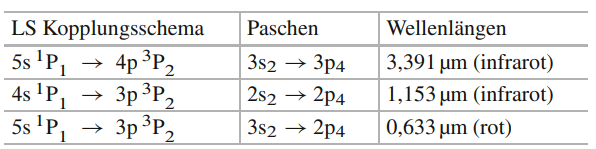
\includegraphics[width=\textwidth]{Bilder/linie.PNG}
    \caption{Übergänge der intensivsten Linien des Neons.\cite{Laser}}
    \label{fig:linie}
\end{figure}

Der gesamte Aufbau eins He-Ne-Laser ist in Abbildung \ref{fig:he} dargestellt.

\begin{figure}
    \centering
    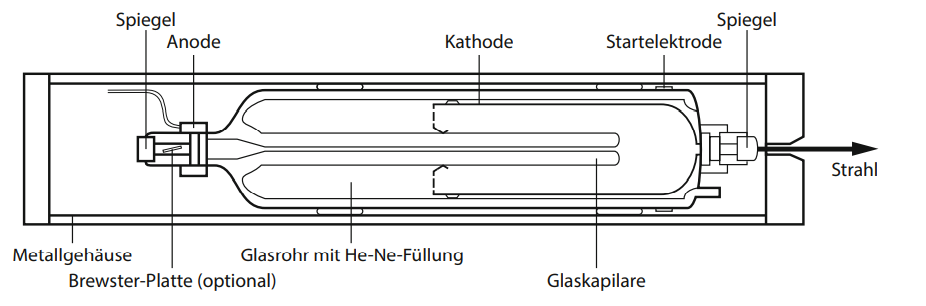
\includegraphics[width=\textwidth]{Bilder/he.PNG}
    \caption{Aufbau eines He-Ne-Lasers.\cite{Laser}}
    \label{fig:he}
\end{figure}


\subsection{Wellenlänge}

Wie bereits erwähnt wird die Wellenlänge des Lasers hauptsächlich durch die Wahl des aktiven Mediums bestimmt. 
Die Wellenlänge des Lichtes kann mit Hilfe eines Gitters bestimmt werden. Dabei lässt sich die Wellenlänge über die Relation
\begin{equation}
    \label{eqn:lamb}
    \lambda = \frac{g\sin{\left(\arctan{\left(\frac{d_k}{L}\right)}\right)}}{k}
\end{equation}
bestimmen. Dabei ist $g$ die Gitterkonstante, $d_k$ der Abstand vom Mittelpukt bis zum k-ten Maximum und $L$ der Abstand zwischen dem Gitter und dem Schirm.

\subsection{Polarisation}

Licht kann unterschiedlich polarisiert sein. Trifft linear Polarisiertes auf einen Polarisationsfilter, so wird in Abhängigkeit des Winkels $\phi$ zwischen Filter und Polarisationsrichtung nur ein Teil des Lichtes durch den Filter gelangen. Die Intensität der durchgelassenen Strahlung lässt sich über das \textit{Gesetz von Malus}
\begin{equation}
    \label{eqn:pol}
    I = I_0\cos^2{(\phi)}
\end{equation}
bestimmen.
%In knapper Form sind die physikalischen Grundlagen des Versuches, des Messverfahrens, sowie sämtliche für die Auswertung erforderlichen Gleichungen darzustellen. (Keine Herleitung)

%(eventuell die Aufgaben)

%Der Versuchsaufbau: Beschreibung des Versuchs und der Funktionsweise (mit Skizze/Bild/Foto)

\section{Durchführung}
\label{sec:Durchführung}


Für den Versuch wird ein Aufbau gemäß Abbildung \ref{fig:aufbau} verwendet.

\begin{figure}
    \centering
    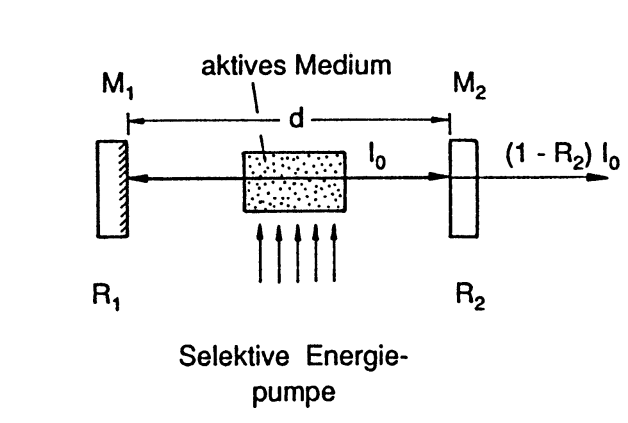
\includegraphics[width=\textwidth]{Bilder/Aufbau.PNG}
    \caption{Schematischer Versuchsaufbau.}
    \label{fig:aufbau}
\end{figure}

Da es im Rahmen des Versuchs, keine Möglichkeit gibt, das Magnetfeld während des Versuchs zu messen, wird der Elektromagent geeicht. Dazu wird die Feldstärke des B-Feldes, mit Hilfe einer in das Feld eingeführten Hall-Sonde, in Abhängigkeit des Stroms gemessen. So kann auch ohne Hall-Sonde, über den Strom auf die Feldstärke des Magneten rückgeschlossen werden.



Für eine möglichst genaue Messung muss der Aufbau zunächst justiert werden. Die Justage wird an der Cd-Lampe begonnen und der Reihenfolge der Bauteile nach durchgeführt. 
Als erstes wird das Licht der Cd-Lampe über ein Objektiv und einer Linse scharf auf den ersten Spalt $S_1$ abgebildet.
Daraufhin wird das Licht in der Linse $L_2$ so gebrochen, dass ein möglichst paralleles Lichtbündel entsteht, welches dann mit wenig Verlust in das Geradsichtprisma fällt. Dazu sollte der Durchmesser des Lichtsbündels die größe des Prismas nicht übersteigen. 
Über die Linse $L_3$ werden die Lichtstrahlen, die das Prisma verlassen, scharf auf den Spalt $S_2$ abgebildet. Über diesen Spalt kann dann eine Selektion der einzelnen Spektrallinien vorgenommen werden. Über die Justage der Linse $L_4$ wird ein scharfes Bild auf die Lummer-Gehrcke-Platte geworfen. Auch hier wird darauf geachtet, dass das Bild der Größe des Eintritts-Prismas entspricht. 
Nun wird ein Polarisator in dem Strahlengang platziert, welcher, je nach Stellung, den jeweiligen Übergang ($\Delta m = \pm1,0$) ausblendet.
Am Ende des Aufbaus ist eine, auf die Lummer-Gehrcke-Platte gerichtete, Kamera angebracht, mit der die aufgespalteten Linien fotografiert werden können. Damit ist der Aufbau und die Justage abgeschlossen und der eigentliche Messvorgang kann beginnen. 


Zuerst wird die rote Linie betrachtet. Dazu wird der Spalt $S_2$ auf die rote Linie geschoben. Durch eine Verschiebung des Spalten kann es vorkommen, dass die folgenden Bauteile erneut nachjustiert werden müssen. Dies gilt auch für die späteren Messungen der blauen Linie.
Daraufhin wird bei ausgeschaltetem B-Feld das Spektrum der roten Linie fotografiert. Das B-Feld wird gemäß Tabelle REF eingestellt und es werden Fotos in Abhängigkeit der Stellung des Polarisationsfliter erstellt. Bei einer Polarisator-Stellung von $\SI{0}{\degree}$ wird das $\sigma$-polarisierte Licht ausgeblendet und bei einer Polarisator-Stellung von $\SI{90}{\degree}$ wird das $\pi$-polarisierte Licht ausgeblendet.
Dieser Vorgang wird analog für die blaue Linie durchlaufen. Auf diese Weise werden also ingesamt sechs Bilder aufgenommen, welche jeweils vom B-Feld und der Stellung des Polarisators abhängen.

 %Was wurde gemessen bzw. welche Größen wurden variiert?
\section{Auswertung}
\label{sec:Auswertung}
Alle Berechnungen werden mit dem Programm \glqq Numpy" \cite{numpy}, die Unsicherheiten mit dem Modul \glqq Uncertainties" \cite{uncertainties}, die Ausgleichsrechnungen mit dem Modul \glqq Scipy" \cite{scipy} durchgeführt und die grafischen Darstellungen über das Modul \glqq Matplotlib" \cite{matplotlib} erstellt.

Die Heizraten der jeweiligen Temperaturverläufe, wie sie in den Tabellen [] und [] zu sehen ist, lassen sich durch 

\begin{equation}
    \Delta b_i = \frac{T_i - T_{i-1}}{\SI{60}{s} }
\end{equation}

darstellen. Daraus lassen sich die beiden mittleren Heizraten 

\begin{align*}
    h_1 &=  \SI{1.360(029)}{\kelvin\per\minute}  \\
    h_2 &=  \SI{1.912(056)}{\kelvin\per\minute} \\
\end{align*}

berechnen. 

Außerdem wird ein Untergrundstrom identifiziert, der über einen Exponetial-Fit der Form 
\begin{equation}
    f(x) = a e^{bx} + c
\end{equation}

beschrieben wird. Dieser Untergrund wird dann von den Werten der beiden Messreihen subtrahiert, damit ein charakteristischer Verlauf des Relaxationsstroms sichtbar wird. 

\subsection{Aktivierungenergie über Polarisationsansatz}

Über den Polarisationsansatz kann, wie im Abschnitt \ref{sec:pol} beschrieben, die Aktivierungenergie $W$ näherungsweise bestimmt werden.
Die so errechneten Werte für die beiden Messreihen ergeben sich zu 
\begin{align*}
    W_{\text{int},1.5} &= \SI{1.46(06)e-19}{\joule} &= \SI{0.91(04)}{\electronvolt} \\
    W_{\text{int},2}   &= \SI{9.4(12)e-20}{\joule} &= \SI{0.59(08)}{\electronvolt} \\
\end{align*}


\subsection{Aktivierungenergie über Stromdichte}

Eine weitere Möglichkeit, aus den Datensätzen einen Wert für die Aktivierungsenergie zu bestimmen, wird im Abschnitt \ref{sec:int} gezeigt. 
Dazu wird eine lineare Regression der Form 

\begin{equation}
    F(T) = \frac{m}{T} + c
\end{equation}

durchgeführt, was die Gleichung 
\begin{equation}
    \ln{\tau} = \ln(\tau_0) + \frac{W}{k_B T}
\end{equation} 
wiederspiegelt.

Damit werden die Aktivierungenergien beider Messreihen zu 

\begin{align*}
    W_{\text{apr},1.5} &= \SI{8.4(5)e-20}{\joule} &= \SI{0.524(033)}{\electronvolt} \\
    W_{\text{apr},2}   &= \SI{9.0(5)e-20}{\joule} &= \SI{0.560(033)}{\electronvolt} \\
\end{align*}

bestimmt.

\subsection{Charakteristische Relaxationszeit}

Die charakteristische Relaxationszeit kann über die Aktivierungenergie bestimmt werden. Mit den aufgenommenen Daten  und den bereits 
errechneten Heizraten kann die Gleichung 
\begin{equation}
    T^2_\text{max} = bW = \frac{\tau(T_\text{max})}{k_B} 
\end{equation} 
verwendet werden, um mit den jeweils maximalen Temperaturen $T_{max,1.5} = \SI{259.2}{\kelvin} $ und $T_{max,2} = \SI{260.5}{\kelvin} $ 
jweils $\tau_0$  für beide Methoden zu bestimmen. \\

Für die Werte des Polarisationsansatzes ergeben sich die $\tau_0$ damit zu 
\begin{align*}
    \tau_{0,1.5} &= \SI{2.5(29)e-12}{\second}\\
    \tau_{0,2}   &= \SI{1.8(21)e-12}{\second}\\ 
\end{align*}
und für den Ansatz über die Stromdichte ergibt sich 
\begin{align*}
    \tau_{0,1.5} &= \SI{1.9(32)e-13}{\second}\\
    \tau_{0,2}   &= \SI{1.4(24)e-13}{\second}\\ 
\end{align*}

Es lässt sich daraus eine Abhängigkeit der Relaxationszeit von der Aktivierungsenergie und der charakteristischen Relaxationszeit beschreiben, die im Plot [] sichtbar ist. Dabei 
werden hier die Werte der Integrationsmethode verwendet und es können die Verläufe der beiden Messreihen verglichen werden. 


\section{Diskussion}
\label{sec:Diskussion}


In Tabelle \ref{tab:zusa} sind die bestimmten Aktivierungsenergien zusammenfassend dargestellt. Laut \cite{Dipol} ist der Literaturwert auf $W_\text{lit} = \SI{0.66}{\electronvolt}$ angegeben. Die jeweiligen Abweichungen sind ebenfalls der Tabelle zu entnehmen. 

\begin{table}
    \centering
    \caption{Zusammenfassung der Ergebnisse.}
    \label{tab:zusa}
    \sisetup{table-format = 1.2}
    \begin{tabular}{S S S S S}
        \toprule
        & \multicolumn{2}{c}{Integration} & \multicolumn{2}{c}{Approximation} \\
        \cmidrule(lr){2-3} \cmidrule(lr){4-5}
        {$\text{mittl. Heizrate} \mathbin{/} \si{\kelvin\per\minute} $} & {$W \mathbin{/} \si{\electronvolt}$} & {$\text{Abw.} \mathbin{/} \si{\percent}$} & {$W \mathbin{/} \si{\electronvolt}$} & {$\text{Abw.} \mathbin{/} \si{\percent}$} \\
        \midrule   
        1.36 & \num{0.91(04)} & \num{38(6)} & \num{0.524(033)} & \num{21(5)}  \\
        1.91 & \num{0.59(08)} & \num{12(11)} & \num{0.560(033)} & \num{15(5)}  \\
        \bottomrule
    \end{tabular}
\end{table}

Es fällt auf, dass die Werte bei der geringeren Heizrate stärker vom Literaturwert abweichen, als die bei der höheren. Das kann auf die Reihenfolge der Messdurchläufe zurückzuführen sein. Im Versuch ist mit der geringeren Heizrate angefangen worden. Da sich erstmal an die Wirkung und Empfindlichkeit der Temperaturregelung gewöhnt werden musste, kann es sein, dass die Heizrate nicht optimal konstant gehalten werden konnte. Zwischen den beiden Methoden lässt sich kein besonders großer Unterschied festellen. Die Ergebnisse der Approximations-Methode bei der ersten Heizrate weichen zwar nur halb so stark ab, dafür ist die Abweichung bei der zweiten Heizrate sogar ein wenig höher. 


Die berechneten Relaxationszeiten weichen mehrere Größenordungen von dem Literaturwert von $\tau_{0,\text{lit}} = \SI{4e-14}{\s}$ ab. 
Da die Aktivierungsenergien exponetiell in die berechnung der Relaxationszeiten eingehen, sorgen bereits kleine Abweichungen für große Abweichungen der bestimmten Relaxationszeiten. 


Bei Betrachtung der Kurvenverläufe des Strom gegenüber der Temperatur fällt ein nachfolgendes Maximum auf. Innerhalb der hier präsentierten Theorie lassen sich diese Verläufe nicht erklären. Jedoch werden zum herleiten der Gleichungen nur die Dipolmomente erster Ordnung betrachtet. Diese zweiten Maxima werden durch Momente höherer Ordnung verursacht. Durch die steigende Temperatur können so Dipole ralaxieren, die eine höhere Coulomb-Barriere überwinden und damit eine höhere Aktivierungsenergie aufbringen müssen. 


Da im Versuch nur mit einer Art Kristall gearbeitet wird, kann kaum auf die Güte des Versuchs im Allgemeinen geschlossen werden. In diesem konkreten Fall aber, kann die Relaxation gut gezeigt werden. Auch eine grobe Bestimmung der Aktivierungsenergien ist möglich. Für eine gute Bestimmung der Relaxationszeiten ist jedoch die Präzision nicht hoch genug.
%Kurze Zusammenfassung der Ergebnisse
%-Vergleich mit Literaturwerten
%-Vergleich mit verschiedenen Messverfahren
%-bei Abweichungen mögliche Ursachen finden
\section{Messdaten}
\label{sec:Messdaten}

\begin{table}
    \centering
    \caption{$TEM_{01}$-Mode}
    \label{tab:TEM01}
    \sisetup{table-format = 2.2}
    \begin{tabular}[t]{S S}
        \toprule
        $l \mathbin{/} \si{\milli\m}$ & $I \mathbin{/} \si{\micro\watt}$ \\
        \midrule

        30 & 0.13   \\
        29 & 0.12   \\
        28 & 0.12   \\
        27 & 0.12   \\
        26 & 0.11   \\
        25 & 0.12   \\
        24 & 0.11   \\
        23 & 0.12   \\
        22 & 0.13   \\
        21 & 0.12   \\
        20 & 0.13   \\
        19 & 0.16   \\
        18 & 0.22   \\
        17 & 0.27   \\
        16 & 0.31   \\
        15 & 0.36   \\
        14 & 0.53   \\
        13 & 0.90   \\
        12 & 1.45   \\
        11 & 2.20   \\
        10 & 3.00   \\
        9 & 4.10    \\
        8 & 5.50    \\
        7 & 7.40    \\
        6 & 9.30    \\
        5 & 11.2    \\
        4 & 13.3    \\
        3 & 15.00   \\
        2 & 16.70   \\
        1 & 18.80   \\
        0 & 17.50   \\

        \bottomrule
    \end{tabular}
    \begin{tabular}[t]{S S}
        \toprule
        $l \mathbin{/} \si{\milli\m}$ & $I \mathbin{/} \si{\micro\watt}$ \\
        \midrule

        -1 & 17.30  \\
        -2 & 16.20  \\
        -3 & 15.30  \\
        -4 & 13.80  \\
        -5 & 11.00  \\
        -6 & 8.90   \\
        -7 & 6.70   \\
        -8 & 4.80   \\
        -9 & 3.50   \\
        -10 & 2.30  \\
        -11 & 1.60  \\
        -12 & 0.90  \\
        -13 & 0.90  \\
        -14 & 0.55  \\
        -15 & 0.32  \\
        -16 & 0.21  \\
        -17 & 0.15  \\
        -18 & 0.12  \\
        -19 & 0.10  \\
        -20 & 0.10  \\
        -21 & 0.09  \\
        -22 & 0.09  \\
        -23 & 0.09  \\
        -24 & 0.08  \\
        -25 & 0.09  \\
        -26 & 0.09  \\
        -27 & 0.09  \\
        -28 & 0.09  \\
        -29 & 0.09  \\
        -30 & 0.08  \\

        \bottomrule

    \end{tabular}
\end{table}



\begin{table}
    \centering
    \caption{$TEM_{00}$-Mode}
    \label{tab:TEM00}
    \sisetup{table-format = 2.2}
    \begin{tabular}[t]{S S}
        \toprule
        $l \mathbin{/} \si{\milli\m}$ & $I \mathbin{/} \si{\micro\watt}$ \\
        \midrule

        30 & 0.13   \\
        29 & 0.12   \\
        28 & 0.12   \\
        27 & 0.12   \\
        26 & 0.11   \\
        25 & 0.12   \\
        24 & 0.11   \\
        23 & 0.12   \\
        22 & 0.13   \\
        21 & 0.12   \\
        20 & 0.13   \\
        19 & 0.16   \\
        18 & 0.22   \\
        17 & 0.27   \\
        16 & 0.31   \\
        15 & 0.36   \\
        14 & 0.53   \\
        13 & 0.90   \\
        12 & 1.45   \\
        11 & 2.20   \\
        10 & 3.00   \\
        9 & 4.10    \\
        8 & 5.50    \\
        7 & 7.40    \\
        6 & 9.30    \\
        5 & 11.2    \\
        4 & 13.3    \\
        3 & 15.00   \\
        2 & 16.70   \\
        1 & 18.80   \\
        0 & 17.50   \\

        \bottomrule

    \end{tabular}
    \begin{tabular}[t]{S S}
        \toprule
        $l \mathbin{/} \si{\milli\m}$ & $I \mathbin{/} \si{\micro\watt}$ \\
        \midrule

        -1 & 17.30  \\
        -2 & 16.20  \\
        -3 & 15.30  \\
        -4 & 13.80  \\
        -5 & 11.00  \\
        -6 & 8.90   \\
        -7 & 6.70   \\
        -8 & 4.80   \\
        -9 & 3.50   \\
        -10 & 2.30  \\
        -11 & 1.60  \\
        -12 & 0.90  \\
        -13 & 0.90  \\
        -14 & 0.55  \\
        -15 & 0.32  \\
        -16 & 0.21  \\
        -17 & 0.15  \\
        -18 & 0.12  \\
        -19 & 0.10  \\
        -20 & 0.10  \\
        -21 & 0.09  \\
        -22 & 0.09  \\
        -23 & 0.09  \\
        -24 & 0.08  \\
        -25 & 0.09  \\
        -26 & 0.09  \\
        -27 & 0.09  \\
        -28 & 0.09  \\
        -29 & 0.09  \\
        -30 & 0.08  \\

        \bottomrule

    \end{tabular}
\end{table}


\begin{table}
    \centering
    \caption{Positionen der Intensitätsmaxima unter Verwendung verschiedner Gitter und Schirm-Gitter Abstände.}
    \label{tab:gitter}
    \sisetup{table-format = 2.1}
    \begin{tabular}[t]{S S S}
        \toprule
        \multicolumn{3}{c}{$g_1 = \frac{1}{600} \si{\milli\m} $, $L = \SI{82}{\centi\m}$} \\
        \cmidrule(lr){1-3}
        {$k$} & {$d_r$} & {$d_l$} \\
        \midrule
        1 & 33.6 & 34.1 \\
        \bottomrule
    \end{tabular}
    \begin{tabular}[t]{S S S}
        \toprule
        \multicolumn{3}{c}{ $g_2 = \frac{1}{100} \si{\milli\m}$, $L = \SI{74}{\centi\m}$ } \\
        \cmidrule(lr){1-3}
        {$k$} & {$d_r$} & {$d_l$} \\
        \midrule
        1 &  4.9  & 4.9   \\
        2 &  9.8  & 9.8   \\
        3 & 14.8 & 14.8   \\
        4 & 20.0 & 19.9   \\
        5 & 25.5 & 25.5   \\
        6 & 31.3 & 31.4   \\
        \bottomrule
    \end{tabular}
    \begin{tabular}[t]{S S S}
        \toprule
        \multicolumn{3}{c}{$g_3 = \frac{1}{1200} \si{\milli\m}$, $L = \SI{29}{\centi\m}$} \\
        \cmidrule(lr){1-3}
        {$k$} & {$d_r$} & {$d_l$} \\
        \midrule
        1 & 34.5 & 34.0 \\
        \bottomrule
    \end{tabular}
    \begin{tabular}[t]{S S S}
        \toprule
        \multicolumn{3}{c}{$g_4 = \frac{1}{80} \si{\milli\m}$, $L = \SI{77}{\centi\m}$} \\
        \cmidrule(lr){1-3}
        {$k$} & {$d_r$} & {$d_l$} \\
        \midrule
        1 & 3.9 & 4.0   \\
        2 & 7.9 & 7.9   \\
        3 & 11.9 & 11.9 \\
        4 & 15.8 & 15.9 \\
        5 & 20.2 & 20.2 \\
        6 & 24.6 & 24.5 \\
        7 & 29.3 &   \\
        \bottomrule
    \end{tabular}
\end{table}

\begin{table}
    \centering
    \caption{Lichtintensität in Abhängigkeit des Filterwinkels.}
    \label{tab:polar}
    \sisetup{table-format = 1.4}
    \begin{tabular}[t]{S S}
        \toprule
        $\phi \mathbin{/} \si{\degree}$ & $I \mathbin{/} \si{\milli\watt}$ \\
        \midrule
        0 & 0.0185  \\
        4 & 0.0510  \\
        8 & 0.115   \\
        12 & 0.21   \\
        16 & 0.33   \\
        20 & 0.44   \\
        24 & 0.62   \\
        28 & 0.78   \\
        32 & 0.95   \\
        36 & 1.11   \\
        40 & 1.32   \\
        44 & 1.53   \\
        48 & 1.62   \\
        52 & 2.00   \\
        56 & 2.20   \\
        60 & 2.35   \\
        64 & 2.50   \\
        68 & 2.60   \\
        72 & 2.70   \\
        76 & 2.75   \\
        80 & 2.85   \\
        84 & 2.85   \\
        88 & 2.90   \\
        92 & 2.80   \\
        \bottomrule
    \end{tabular}
    \begin{tabular}[t]{S S}
        \toprule
        $\phi \mathbin{/} \si{\degree}$ & $I \mathbin{/} \si{\milli\watt}$ \\
        \midrule
        96 & 2.75   \\
        100 & 2.70  \\
        104 & 2.55  \\
        108 & 2.45  \\
        112 & 2.35  \\
        116 & 2.10  \\
        120 & 1.90  \\
        124 & 1.75  \\
        128 & 1.55  \\
        132 & 1.40  \\
        136 & 1.20  \\
        140 & 0.97  \\
        144 & 0.81  \\
        148 & 0.64  \\
        152 & 0.48  \\
        156 & 0.33  \\
        160 & 0.23  \\
        164 & 0.13  \\
        168 & 0.0710    \\
        172 & 0.0215    \\
        176 & 0.0073    \\
        180 & 0.0190    \\

        \bottomrule

    \end{tabular}
\end{table}


\begin{table}
    \centering
    \caption{Intensitätsmessungen bei konkav-konkaver Spiegelkonstallation mit jeweilgem Krümmungsradius $r = \SI{1400}{\milli\m}$ .}
    \label{tab:kon_kon}
    \sisetup{table-format = 1.2}
    \begin{tabular}[t]{S S}
        \toprule
        $L \mathbin{/} \si{\centi\m}$ & $I \mathbin{/} \si{\milli\watt}$ \\
        \midrule
        63 & 3.8    \\
        65 & 3.95   \\
        67 & 4.10   \\
        69 & 3.77   \\
        71 & 3.90   \\
        73 & 3.90   \\
        75 & 3.85   \\
        77 & 3.70   \\
        79 & 3.10   \\
        81 & 3.75   \\
        83 & 3.90   \\
        85 & 3.45   \\
        87 & 3.90   \\
        89 & 3.70   \\
        95 & 3.75   \\
        100 & 3.65  \\
        105 & 3.60  \\
        144 & 1.40  \\
        154 & 1.40  \\
        164 & 1.40  \\
        174 & 2.20  \\
        184 & 1.50  \\
        194 & 2.15  \\

        \bottomrule

    \end{tabular}
\end{table}

\begin{table}
    \centering
    \caption{Intensitätsmessungen bei plan-konkaver Spiegelkonstallation mit Krümmungsradius $r = \SI{1400}{\milli\m}$ .}
    \label{tab:plan_kon}
    \sisetup{table-format = 1.2}
    \begin{tabular}[t]{S S}
        \toprule
        $L \mathbin{/} \si{\centi\m}$ & $I \mathbin{/} \si{\milli\watt}$ \\
        \midrule
        50 & 2.60   \\
        55 & 1.60   \\
        60 & 1.50   \\
        65 & 1.55   \\
        70 & 1.70   \\
        75 & 1.80   \\
        80 & 2.00   \\
        85 & 2.15   \\
        90 & 2.15   \\
        128.5 & 4.00    \\

        \bottomrule

    \end{tabular}
\end{table}

\printbibliography{}

\end{document}
